% This is LLNCS.DOC the documentation file of
% the LaTeX2e class from Springer-Verlag
% for Lecture Notes in Computer Science, version 2.4
\documentclass{llncs}
\usepackage{llncsdoc}

\usepackage[T1]{fontenc}
\usepackage[latin1]{inputenc}
\usepackage[table, svgnames]{xcolor} 
\usepackage{color} 
\usepackage{url}
\usepackage{graphicx, array, blindtext}
\usepackage[tight,footnotesize]{subfigure}
\usepackage{mdframed}
\usepackage{latexsym}
\usepackage{boxedminipage}
\usepackage{ amssymb }
\usepackage[normalem]{ulem}
\usepackage{flushend}

\usepackage{ocgx}
\usepackage{tikz}
\usetikzlibrary{ocgx}

\setlength\floatsep{1\baselineskip plus 3pt minus 2pt}
\setlength\textfloatsep{1\baselineskip plus 3pt minus 2pt}
\setlength\intextsep{1\baselineskip plus 3pt minus 2 pt}
%
\begin{document}

\begin{center}

\LARGE \textbf{Why are program analysis tools difficult to understand?} \\
\Large A tool (mis)communication theory and adaptive approach for supporting developers during tool use \\[2.0em]

\end{center}

\begin{center}
	Brittany Johnson\\[1.0em]
	NC State University \\
	bijohnso@ncsu.edu
	
\end{center}


\vspace{2pt}

\begin{abstract}
	
\end{abstract}

\vfill

%\rule{\textwidth}{1pt}
%\begin{flushleft}
%\large\itshape
%\begin{tabular}{@{}l}
%{\Large\upshape\bfseries Springer}\\[8pt]
%Berlin\enspace Heidelberg\enspace New\kern0.1em York\\[5pt]
%Barcelona\enspace Budapest\enspace Hong\kern0.2em Kong\\[5pt]
%London\enspace Milan\enspace Paris\enspace\\[5pt]
%Santa\kern0.2em Clara\enspace Singapore\enspace Tokyo
%\end{tabular}
%\end{flushleft}


%
%{\tt svserv@vax.ntp.springer.de}\hfil first try the \verb|help|
%command.
%



%
\newpage
\tableofcontents
\newpage
%

% TODO update ToC with page numbers!

\section{Introduction}


\fbox{
	\parbox{\textwidth}{If program analysis \emph{tool use} is a form of \emph{communication} and \emph{inability to resolve} notifications is \emph{miscommunication}, tools can adopt a theory similar to \emph{constructivism} where tools can \emph{approximate} individual developer's \emph{conceptual knowledge} to adapt notifications, leading to \emph{reduced time and effort} required for developers to understand and resolve tool notifications.
		}
	}
%


\section{Research Significance}

\subsection{What are program analysis tools?}
Program analysis tools are tools designed to aide developers when developing software by automating the writing, analysis, and modification of source code.
Often, program analysis is discussed as synonymous with static analysis~\cite{nielson2015principles}. 
For the purpose of my research, I define a program analysis tool as a tool that performs program analysis, whether it be static or dynamic analysis.
Examples of program analysis tools include, but are not limited to, static code analyzers, code coverage tools, code smell detectors, and refactoring tools~\cite{adolph2011using, Murphy-Hill:2010:Ambient,ge2012reconciling}.
In the following sections, I will define and discuss static analysis and dynamic analysis tools separately; the reader should note that although we discuss static and dynamic analysis separately, it is not uncommon to find program analysis tools that combine static and dynamic analysis~\cite{ernst2003static}.                                                

\subsubsection{Static Analysis Tools}

Static analysis tools are designed to aide developers when developing software by statically analyzing source code, pre-runtime, and providing the developer with feedback about the state of their code~\cite{ernst2003static}.
Typically, static analysis works by examining the current state of the program and then predicting and reporting how the program may react in that state at runtime. Static analyses are often more conservative than dynamic analyses; this is to reduce the potential for false positives, as in most cases static analysis cannot say with 100\% certainty what will happen during run-time. 
Examples of static analysis tools include defect detectors, such as FindBugs, compilers, code smell detectors, and refactoring tools.

Let's use the example of FindBugs,~\footnote{http://findbugs.sourceforge.net/factSheet.html} an open source static analysis tool, to better understand how static analysis tools work. FindBugs statically analyzes code to report potential defects. FindBugs determines the potential for defects using \emph{bug patterns}


\subsubsection{Dynamic Analysis Tools}

Dynamic analysis tools are designed to aide developers when developing software by analyzing source code during run-time and providing the developer with feedback about runtime behavior~\cite{ernst2003static}.
Dynamic analysis works by executing the program and then making observations about program execution; because dynamic analysis runs the code, it is typically more precise than static analysis. Though dynamic analysis can produce more precise results in a similar amount of time as static analysis, dynamic analysis is less likely to generalize to future executions.
Examples of dynamic analysis tools include testing, code coverage, and profiling tools.

% TODO make sure to mention idea of test suite may not be characteristic of all possible executions of program (relates back to generalizability of dynamic analyses)
Let's use the example of EclEmma, an open source dynamic test and code coverage tool, to better understand how dynamic analysis tools work.

\subsection{How do they communicate?}

\subsection{What do they communicate about?}

%\subsubsection{What are programming concepts?}

\subsection{How does tool communication relate to verbal communication?}
%\subsubsection{Model of communication \& miscommunication}
%\subsubsection{Relationship to tool use}

\subsection{Why don't developers use program analysis tools?}
% interactive interviews (icse)

\subsection*{Motivating Example}
% merge motivating examples from icse and fse papers into one big example (make sure detailed but say what I mean!)
\begin{figure} 
	\centering
	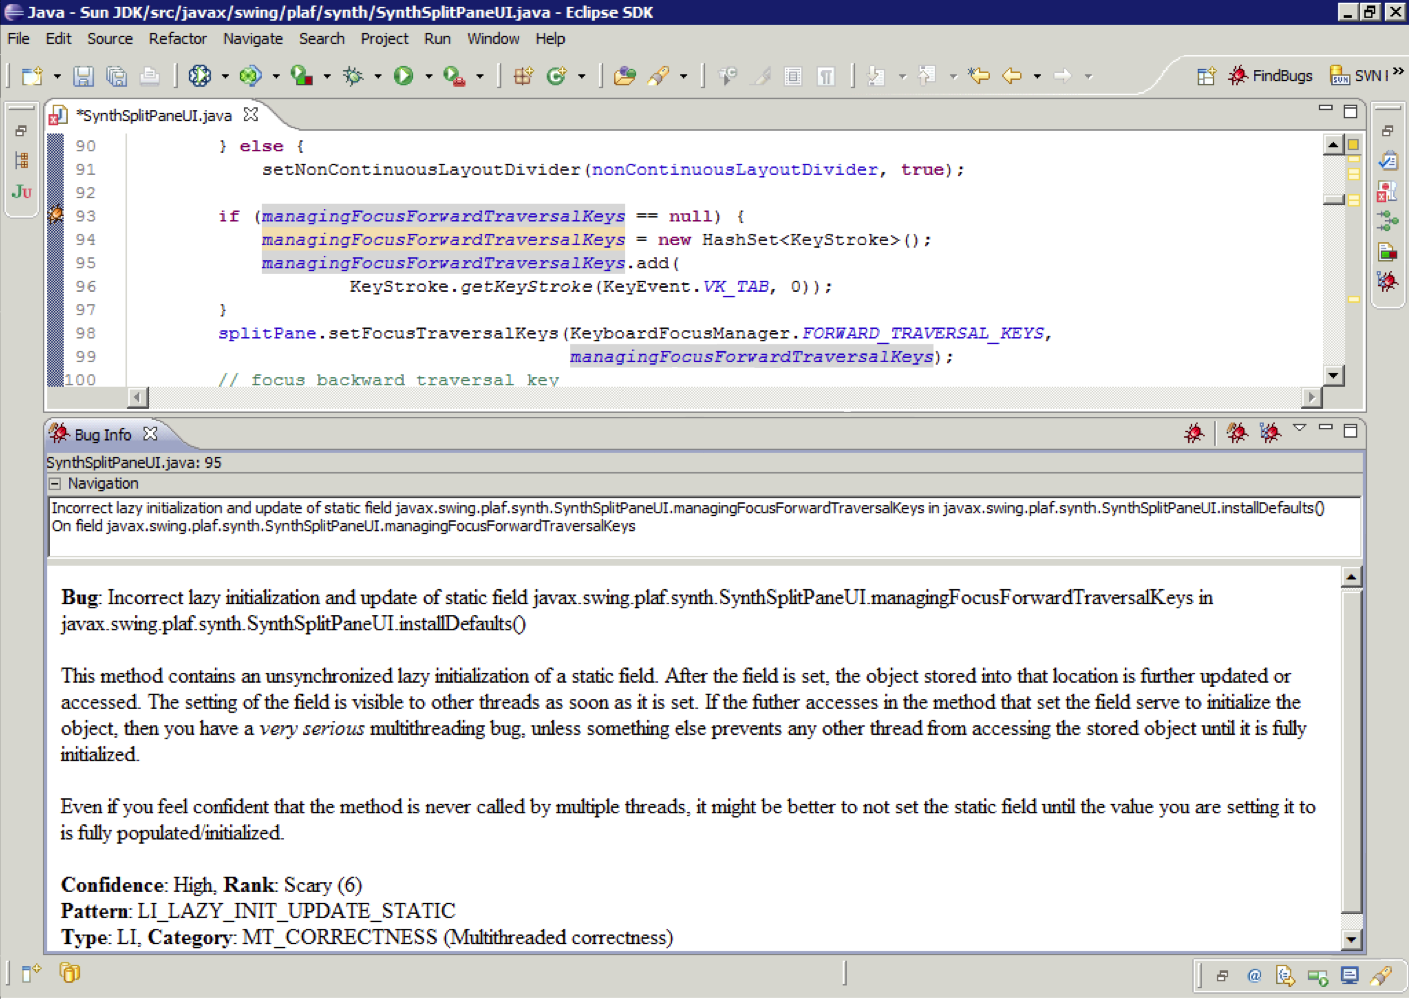
\includegraphics[width=\textwidth]{figs/eclipse.png}
	\caption{Findbugs notification in the Eclipse IDE concerning multi-threading.}
	\label{fig:eclipse}
\end{figure}

Valerie is a software developer at a start-up company. She primarily writes Java code, though she did not learn to program in Java, and uses the Eclipse Integrated Development Environment (IDE). In her spare time, she builds her knowledge of Java programming concepts by contributing to open source software and using tools that provide feedback about the code she writes. While modifying code in the Sun JDK source code repository, she contributes code that results in the notification shown in Figure~\ref{fig:eclipse}. She has experience using FindBugs, so she is familiar with some of the ways FindBugs communicates. For example, she knows that an orange bug icon indicates a \textit{scary} bug and that by clicking the bug icon she can gain access to more information about the bug.

As she explores the information provided by FindBugs, she realizes that despite her experience with FindBugs, she is having difficulty determining how to resolve the notification. She first attempts to use what knowledge she does have regarding multi-threading, which she accrued from struggling with and resolving compiler synchronization warnings, to better understand the problem. However, she is unfamiliar with the concept central to the notification in Figure~\ref{fig:eclipse} (lazy initialization). Though the notification tells her that the problem relates to multi-threading, she is unable to make a connection between her knowledge regarding multi-threading and the message FindBugs is attempting to communicate and therefore cannot resolve the notification without outside help. As done previously with compiler synchronization notifications, she toggles between the web and her IDE to understand and resolve the notification.

% TODO compiler synchronization notification??

\begin{figure} 
	\centering
	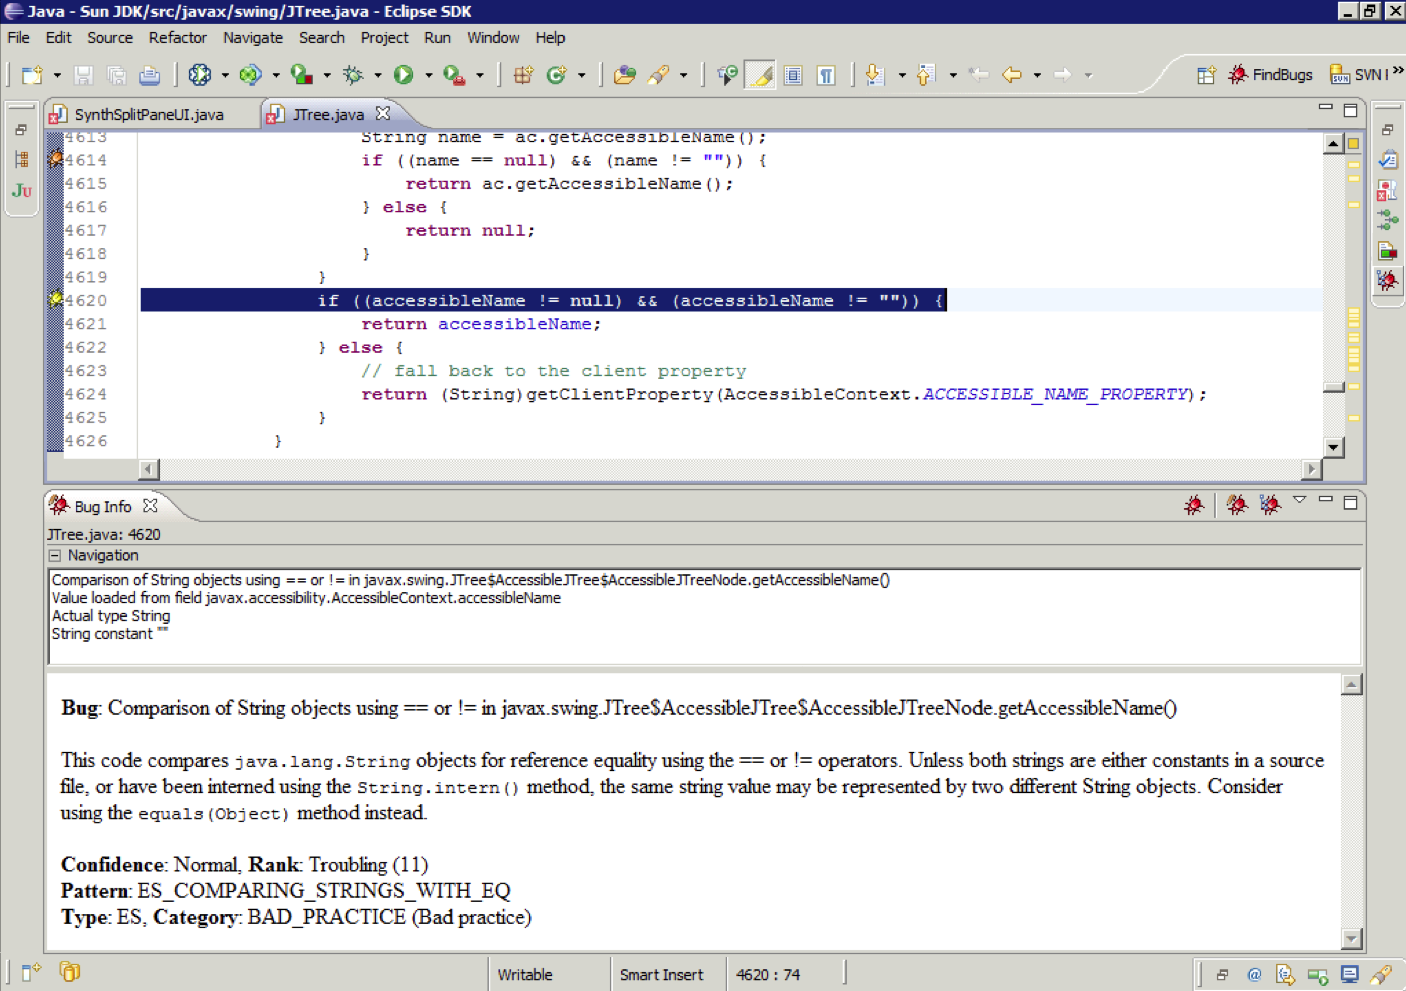
\includegraphics[width=\textwidth]{figs/eclipse-2.png}
	\caption{Findbugs notification in the Eclipse IDE on checking string equality.}
	\label{fig:eclipse2}
\end{figure}

One goal developers have when using tools like FindBugs is to find and resolve defects, which requires the ability to interpret the notifications provided by the tools. Valerie's secondary goal when using tools was to learn more about Java programming concepts. She found, however, that some notifications are better at communicating problems while contributing to knowledge than others. For example, when first learning how to work with strings in Java, Valerie encountered the notification in Figure~\ref{fig:eclipse2}. The first time she encountered the problem she was able to understand and resolve the notification. Looking back, she realizes this was because the notification in Figure~\ref{fig:eclipse2} filled in gaps in her own knowledge of the concept by informing her \emph{why} what she was doing was wrong and \emph{how} she can fix it.

Because the tools Valerie uses have no notion of with what she does and does not know, some notifications are able to communicate effectively, while others run the risk of a miscommunication. Based on the challenges developers may encounter, like the ones Valerie encountered, I propose a tool miscommunication theory that can be used to inform the design of developer tools, such as FindBugs.

% TODO need something relevant to cross-tool!

\section{A Tool Miscommunication Theory}
%session study (fse)

\section{An Approach for Modeling Developer Knowledge}
%modeling approach (vlhcc)

\subsection{Using Concept Inventories to Assess Concept Knowledge}


\subsection{Using Public Git Repositories to Predict Concept Knowledge}


\section{A Proposed Approach for Notification Adaptation}
% bespoke paper (focused on notifications - fse)


\section{Experiments \& Evaluations}

% generalizability assessment (other concepts)
% study 1: apply model to other concepts; do models differ based on concept? Is there some unifying factor that ties together conceptts per model?
% study 2: predicting knowledge on new set of developers for concepts; how well do models perform on other data? how well does it scale?

% notification adaptations
% study 1: design notifications based on existing research; user study to determine which are better for which group (and maybe some participatory design)
% tool: automatically apply predicted knowledge to adapt
% study 2: compare performance between our tool and FindBugs

\section{Related Work}


\section{Project Plan}


\section*{Acknowledgments}


\bibliography{main.bib}

%
%\begin{thebibliography}{[MT1]}
%%
%\bibitem[CE1]{clar:eke}
%Clarke, F., Ekeland, I.:
%Nonlinear oscillations and
%boundary-value problems for Hamiltonian systems.
%Arch. Rat. Mech. Anal. 78, 315--333 (1982)
%%
%\bibitem[CE2]{clar:eke:2}
%Clarke, F., Ekeland, I.:
%Solutions p\'{e}riodiques, du
%p\'{e}riode donn\'{e}e, des \'{e}quations hamiltoniennes.
%Note CRAS Paris 287, 1013--1015 (1978)
%%
%\bibitem[MT1]{mich:tar}
%Michalek, R., Tarantello, G.:
%Subharmonic solutions with prescribed minimal
%period for nonautonomous Hamiltonian systems.
%J. Diff. Eq. 72, 28--55 (1988)
%%
%\bibitem[Ta1]{tar}
%Tarantello, G.:
%Subharmonic solutions for Hamiltonian
%systems via a $\bbbz_{p}$ pseudoindex theory.
%Annali di Matematica Pura (to appear)
%%
%\bibitem[Ra1]{rab}
%Rabinowitz, P.:
%On subharmonic solutions of a Hamiltonian system.
%Comm. Pure Appl. Math. 33, 609--633 (1980)
%\end{thebibliography}
%


\bibauthoryear
%
\end{document}
